\clearpage
\chapter{Introduction}
\label{sec:intro}
The execution of experiments has accompanied humanity throughout its evolution as a cornerstone in the expansion of its knowledge. In particular due to the ever-growing complexity of research, the long term documentation of experimental procedures has become as necessity for a sound exchange of scientific results. However, this is based on the possibility to record the experimental purpose, execution and findings in an exact, comprehensive manner and without bias of any kind. Nowadays, tedious manual scripture has largely been replaced by digital information, making information easier to be transferred, retrieved and duplicated. Therefore, modern scientific research relies mainly on the acquisition and storage of this digitized data. Although raw recording data can be easily stored and disseminated with modern technologies, interpretation of research data is not straightforward as datasets are highly diverse between, and often even within, scientific areas. This inhomogeneity depends highly on the respective field. In areas that require large experimental setups, such as particle physics or high field FMRI, there are only few data formats established by the community and companies that produce the corresponding tools, e.g., the \code{root} format \citep{Brun_1996} and the NIfTI file format. In other fields the diversity of data is larger as scientific methods and objectives require more diverse approaches. Unification would require large-scale coordination within the community and  would imply additional overhead on the level of each experiment. A number of initiatives try to screen, collect and evaluate data and metadata approaches within and across communities. Some examples here are the Human Brain Project\footnote{HBP, \url{https://www.humanbrainproject.eu/en/}} (HBP), which develops a platform to gather data from all neuroscientific areas. The German national research data infrastructure\footnote{NFDI, \url{https://www.dfg.de/foerderung/programme/nfdi/}} is a recent initiative for systematic and sustainable research data management within and across disciplines. However, often such a top-down approach focuses on the few common features of datasets, where it is typically already a challenge to define a set of basic minimal metadata to superficially describe a dataset. Much less attention is devoted to the problem of obtaining an in-depth description of a specific dataset that is consistent with similar data. In light of the complexity of such in-depth metadata providing standardized tools and workflows is a prerequisite for the implementation of sustainable data and metadata management on laboratory level. This permits the integration of data and metadata on a detailed level in a standardized structure, which can later be integrated in large scale infrastructure projects.\\

The diversity in data modalities and file formats promotes a heterogeneity in data analysis steps and tools used for the extraction of scientific findings. Almost 700\footnote{697 results for a query of resource type = 'resource' and 'software resource' and 'data analysis software' and keyword='analysis', accessed on 26.08.2019} data analysis software tools are registered with SciCrunch\footnote{SciCrunch, \url{https://scicrunch.org/}}, a curated repository of scientific resources that includes tools, databases and core facilities with a focus on data analysis in biomedical research. Despite this large set of indexed software tools being searchable as well as citable, many scientific findings have been found to lack reproducibility \citep{Ioannidis_2005,Ioannidis_2007,Baker_2016,Eisner_2018}. One reason for this might be usage of custom code and the neglect of tracking processing and analysis circumstances (provenance tracking). Other reasons might be the inaccessibility of the original data, e.g., due to loss of the original files, deprecated formats or undocumented data selection criteria.\\

This issue has gained more attention in recent time and started a scientific debate about the need for reproducibility of scientific insights, resulting in a number of publications evaluating the reproducibility of published findings (\cref{fig:intro_reproducibility}).
Within this debate, the terms replicability and repeatability \citep{Plesser_2018} have been used to describe different aspects of reproducibility. However, the definitions of all three terms are typically limited to a small scientific community, since the restrictions by the methods used (e.g., laboratory equipment versus human subjects versus scientific simulation software) do not permit a direct translation to other areas. This aggravates the communication on this topic across communities and potentially delays the development towards a more mature awareness of reproducibility in some scientific fields.\\


\begin{figure}[h!]
 \centering
 \includesvg[width=0.7\textwidth]{figures/introduction/trends}
 \caption[Reproducibility related publications]{Reproducibility related publications. Depicted  are publications registered by PubMed\textsuperscript{$\alpha$} that are related to the keywords reproducibility, replicability, repeatability, and reproducibility in combination with neuroscience. Plotted is the fraction of matching publications per year with respect to the total number of registered publications of the same year. Some fractions related to individual keywords were down scaled for better visualization (see legend). Data were extracted using \citet{Corlan_2004}. \small\textsuperscript{$\alpha$} PubMed, \url{https://www.ncbi.nlm.nih.gov/pubmed/}}
 \label{fig:intro_reproducibility}
\end{figure}

While reproducibility is a topic that emerged in the scientific literature already in 1990, especially in the neurosciences it has been relatively unattended and is only recently growing in actuality (\cref{fig:intro_reproducibility}). In addition to the terminology differences described above, the setting of the neurosciences between biology, engineering, physics, chemistry, computer sciences and mathematics might be another reason for this delay. This interdisciplinarity can demand additional communication between neuroscientists and thereby prevent the rigorous questioning of the reproducibility of findings. Another reason might be the relative young age of neuroscience compared to more established scientific fields. This comes with the delayed development of concepts, tools and standards, accompanied by a community awareness of the reproducibility subject.

To address the issue of reproducibility from the perspective of the availability of data, \citet{Wilkinson_2016} defined the FAIR principles. These introduce guidelines for handling research data and metadata and are summarized in four key points. Research data should be made Findable, Accessible, Interoperable and Reusable to be of sustainable value for the scientific community.\\

In this thesis we present and discuss approaches for data and metadata management in the context of these FAIR principles. We focus on efficient and robust handling of research data from its acquisition to analysis with the aim of easy implementation and the usability by individual scientists as well as laboratory-scale collaborations. The presented examples are set in the field of neuroscience, but many concepts, approaches and tools are of generic nature and can therefore be transferred to other scientific disciplines. 



\section{Data and metadata models}
Standardization of data and metadata is a fundamental requirement for the usability of research data. This work is based on two common, generic models for data and metadata representation and storage. Both software projects are developed and maintained by the German Neuroinformatics Node\footnote{G-Node, \url{http://www.g-node.org/}} (G-Node), which is an organization that aims to improve the infrastructure for data access, storage and analysis with an emphasis on the field of electrophysiology. These tools form the basis for the data and metadata acquisition workflows presented in this thesis.

\subsection{Hierarchical metadata in the \software{odML} model}
\label{sec:odml}

The open metadata Markup Language\footnote{\software{odML}, \url{https://github.com/G-Node/python-odml}, RRID:SCR\_001376} (\software{odML}) is a versatile hierarchical framework for the representation and storage of metadata \citep{Grewe_2011}. While it was originally designed for electrophysiological metadata, its generic structure makes it also applicable to other scientific contexts.\\

\begin{figure}[hbt!]
    \centering
    \includestandalone[mode=image|tex, width=0.7\textwidth, obeyclassoptions=true]{./figures/introduction/odML_structure}
    \caption[\software{odML} structure and objects]{\software{odML} structure and objects. \software{odML} provides three objects for metadata organization: The \software{odML} \code{Document} forms the basis of a hierarchy for metadata storage. It can link to a number of \software{odML} \code{Sections}. \code{Sections} are used to build a hierarchical structure and to provide context and relation between metadata. Each \code{Section} can link to multiple \code{Properties}. These contain the actual metadata values accompanied by essential information providing the context for interpretation of the values.}
    \label{fig:intro_odML_structure}
\end{figure}

\begin{figure}[hp]
    \centering
    \scalebox{1}{
    \includesvg[width=\textwidth, pretex=\relscale{0.8}]{./figures/introduction/odML_DataModel_escus}}
    \caption[\software{odML} model versions]{\software{odML} model versions. Illustrated are \software{odML} version 1.3 (A) and version 1.4 (B). Each box represents an entity defined by the data model and is color coded. Connections between entities are illustrated using the UML aggregation relation where a diamond denotes the target of a connection; the numbers at source and target denote the cardinality of each entity in the connection. \code{Documents}, \code{Sections} and \code{Properties} can link to multiple of their child attributes, whereas each object has exactly one parent objects, generating a branching, hierarchical structure. The \code{Document} additionally contains attributes to store the author, the version, the generation date and the corresponding repository reference. The \code{Section} is a container for its child \code{Sections} and \code{Properties}. The \code{Property} name acts as key associated to the actual metadata value stored. In \software{odML} version 1.3 the value information is stored in dedicated \code{Value} objects, whereas in in \software{odML} version 1.4 this feature is integrated into the \code{Property} object. Here, the \code{Property} provides supplementary essential information for the interpretation of the metadata value which was previously stored in the dedicated \code{Value} object in \software{odML} version 1.3. In \software{odML} version 1.4 each object has an identifier (\code{id}) for unique identification across files.}
    \label{fig:intro_odML_model}
\end{figure}

The basic concept is to use a tree-like structure of \code{Sections} to store metadata as \code{Properties} (extended key-value pairs) in a common \code{Document} (\cref{fig:intro_odML_structure}). The \code{Document} captures information about the metadata collection: the author of the collection, the date of generation, a custom version specifier and a custom reference repository. The hierarchical structure of the collection is formed by \code{Sections} which can be concatenated to build the branches of a tree structure (\cref{fig:intro_odML_model}). Here, each \code{Section} carries information about the subset of metadata it contains in form of a \code{Section} \code{name} providing a brief categorization, a \code{definition} extending on the category typically in form a complete sentence, and a \code{type} for grouping across \code{Sections}. Additionally, a \code{Section} can also point to an external \code{repository} or \code{reference} (e.g., a data base) or \code{link} to or \code{include} parts of other \software{odML} structures. The \code{Property} name provides the key corresponding to the stored metadata values. Each \code{Property} contains a list of value entries and gathers the corresponding metadata as its \code{Property} attributes. 
All context information provided by a \code{Property}, i.e. data type (\code{dtype}), physical \code{unit}, \code{uncertainty} and \code{value origin}, is common to all values stored within that \code{Property}.  Similar to the \code{Section} also the \code{Property} can carry a human-readable \code{description} of the values contained and can also \code{reference} to an external location. The value of a \code{Property} can also depend on another \code{Property} (\code{dependency}) or another  value (\code{dependency\_value}). All \software{odML} objects carry a universally unique identifier for unique identification of odML entities even across unrelated files to ensure comprehensive provenance tracking. This permits the referencing and inclusion of \software{odML} objects across files and projects.\\



\begin{figure}[hp]
 \centering
 \scalebox{0.45}{
 \includesvg[width=2.2\textwidth,pretex=\relscale{1.6}]{./figures/introduction/odML_example}}
 \caption[Example \software{odML} structure]{Example \software{odML} structure. The \software{odML} structure contains metadata from an experiment involving a subject that generates a force. The metadata related to this collection itself are denoted in the \software{odML} \code{Document}, e.g., the author. The two top-level \code{Sections} separate subject and recording setup. Here, the recording setup is characterized by two \code{Properties}: the maximum recordable force and the supported sampling rates, consisting of a list of values. The subject is characterized by its species and weight. The training information is described one level below in a \code{Section} named Training. Here the training is characterized solely by a start and end date.}
 \label{fig:intro_example_odml_structure}
\end{figure}

Based on the presented \software{odML} objects, we can design a small example structure for capturing metadata of an experiment involving a subject and a force recording device (\cref{fig:intro_example_odml_structure}). For example, the metadata can be grouped on a first level of \code{Sections} into hardware related or non-hardware related metadata. Here, this implies the generation of two first level \code{Sections}, one for the description of the subject and one for the description of the recording device. On the next level each of these groups can be separate more detailed aspects of the experiment. Here, we only track two aspects of the recording device: the upper limit of the force that can be recorded (\code{Property} with \code{name} Maximum Force) and the supported sampling rates of the device (\code{Property} with \code{name} 'Sampling Rates'). The corresponding value entries to the keys provided by the \code{Property names} are of type \code{list} as \software{odML} supports the capture of multiple values belonging to a \code{Property}. In this example four different sampling rates are supported, sharing the data type, unit, description and all additional attributes of the \code{Property}.
The subject is described by two \code{Properties}, the species and its weight, which are accompanied by the required data type specification and an optional corresponding unit specification. Finally, we also track metadata about the training the subject in a separate subsection of the \code{Section} that describes the subject. Here, the training is solely defined by a start and end date, captured in two corresponding \code{Properties}.

This small example demonstrates how \software{odML} objects can be used to build a hierarchical metadata structure and group information in a logical way. The additional attributes of \code{Sections} and \code{Properties} provide contextual information for the plain metadata values and are essential for the interpretability of the metadata collection. The same concepts  as presented here can be used to build full-sized metadata collections capturing metadata of complex experiments (see \cref{sec:metadata}). For example in the presented example next steps could comprise the addition of more information about the subject in additional \code{Properties} to capture the age, gender, handedness, etc or add additional \code{Sections}, e.g., for describing details related to the recording data (recording date, filenames, etc) or preprocessing steps (filtering, offset removal, etc).




\paragraph{Model revisions}
\label{sec:odml_model_revision}
The projects presented in this thesis rely on different versions of the \software{odML} library. Here we present the main differences between the \software{odML} version 1.3 to and the current \software{odML} version 1.4.
In order to simplify the usage of the odML framework two major changes were introduced in \software{odML} version 1.4. The first change was the merging of \code{Value} and \code{Property} entities (compare \ref{fig:intro_odML_model}A and B). Previously, each \code{Property} required at least one child \code{Value}. In version 1.4. this restriction is lifted, as \code{Properties} can contain an empty list of values. The merge of the two objects prevents value ambiguities within a \code{Property} and reduces the effective file size since the value dependent attributes ("unit", "uncertainty", "data type" and "reference") are defined only once for a set of values. Second, \software{odML} entities now contain a universally unique identifier ("id"), an auto-generated identifier with extremely low collision probability. Compatibility for odML files using the old format version is ensured via automatized conversion functionality.

\paragraph{Additional features}
The \software{odML} core library provides an in-built mechanism to search and retrieve \code{Sections}, \code{Propertie}s or values within a \code{Document}. The need to consistently search for metadata entities across \code{Document}s from different sources led to the development of an export feature of \software{odML} metadata to the Resource Description Framework (RDF) format\footnote{\url{http://www.w3.org/TR/rdf-primer}}, a general and widely used storage format of graph databases. Multiple \software{odML} files exported to RDF can be loaded into any graph database supporting RDF and will be combined into a single graph. Moreover, while XML is the default storage format, \software{odML} additionally supports storing the metadata in the text based file formats JSON\footnote{\url{https://json.org}} and YAML\footnote{\url{https://yaml.org}}. JSON is a de-facto data exchange standard between web based and standalone computer applications. The support of JSON makes \software{odML} metadata more easily consumable in machine-only workflows through modern applications. Since both XML and JSON primarily aim at machine-readability, their structure is not easily readable by humans. \software{odML} also supports the export to the YAML file format to provide a human readable text format of the raw metadata files.

For visualization and manipulation of metadata files, \software{odML} comes with a native \software{odML} GUI (odml-ui\footnote{\url{https://github.com/G-Node/odml-ui}}). The GUI provides a visual representation of the hierarchical structure for navigation and editing of individual metadata entries.


\subsection{Generic data organization via the \software{Nix} model}
The \software{Nix} model is a format to store and represent combined data and metadata in a common framework. For this six generic data objects are defined and combined with an \software{odML} based metadata structure. The \software{Nix} model is provided with a C++ reference implementation\footnote{nixio \software{C++}, \url{https://nixio.readthedocs.io},  RRID:SCR\_016196} and bindings for Java and \software{Matlab}. An independent Python implementation is provided\footnote{nixio / nixpy, Python, \url{https://pypi.org/project/nixio/}} with version $1.5.0b3$ being considered here.

\begin{figure}[hbtp]
 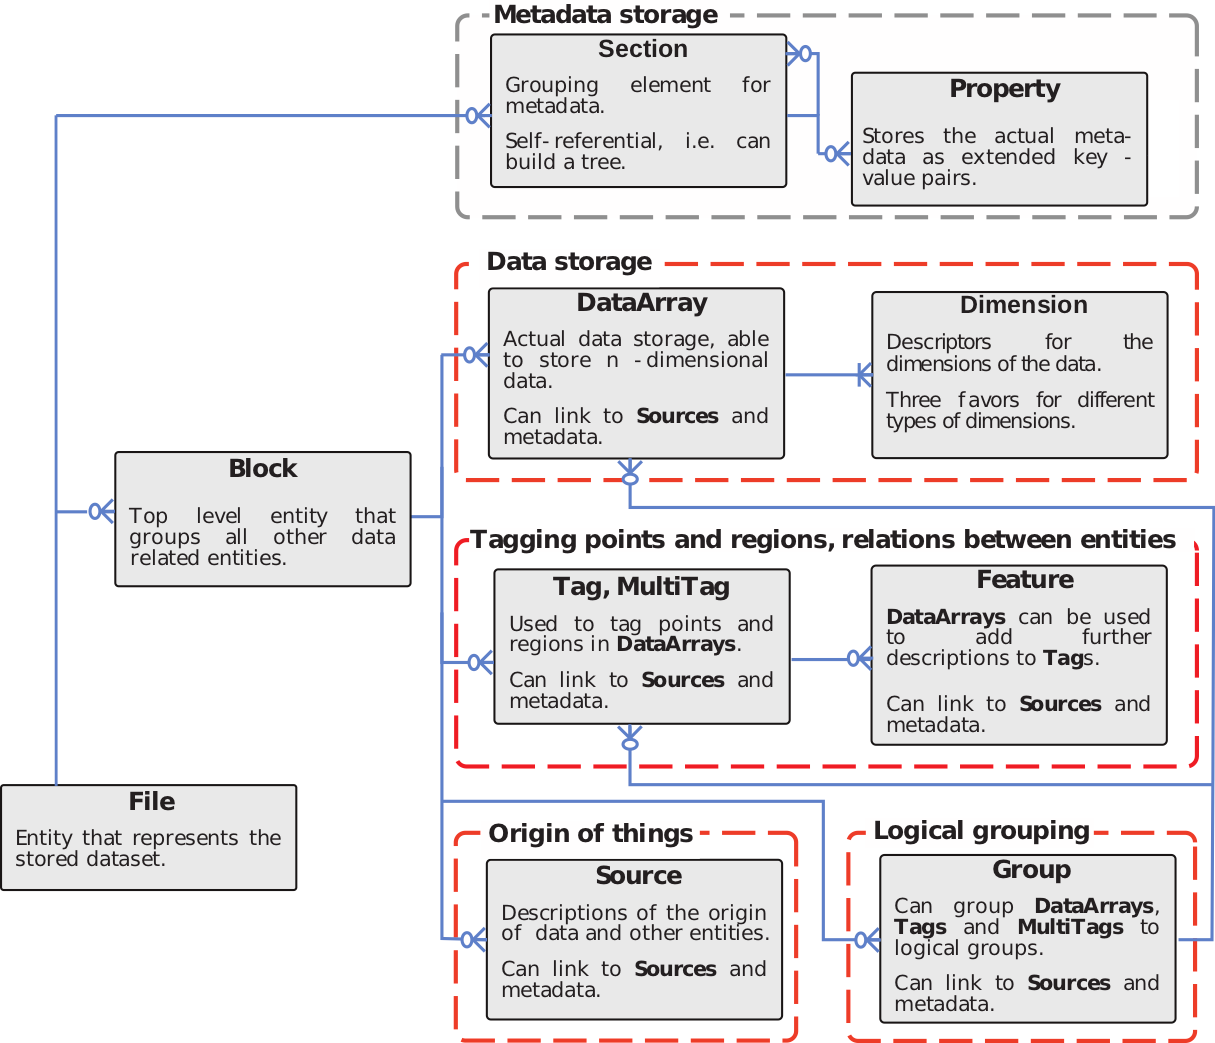
\includegraphics[width=\textwidth]{./figures/introduction/data_model_brief_adapted}
 \caption[\software{Nix} model objects]{\software{Nix} model objects. The model consist of objects for storing data and metadata and relations between these. Metadata is captured in a \software{odML} based structure. Additionally, six objects are implemented to capture data and relation between these. The main data object (\code{DataArray}) stores multidimensional data and captures the physical attributes of the data using \code{Dimension} objects. \code{Tag}s and \code{Multitag}s are used to label a subset of the data contained in a \code{DataArray} and can provide supplementary information using \code{Feature} objects. Furthermore, \code{Group} objects can be used to represent logical relations between objects and \code{Source} objects provide background information about the origin of the data. \code{Block}s and \code{File}s represent a complete dataset and file, respectively. Each of the data objects (except \code{Dimension}s) can link to a corresponding metadata \code{Section} providing additional information specific to that data object. Figure adapted from \software{Nix} documentation (\url{https://nixio.readthedocs.io/en/latest/data_model.html}).}
 \label{fig:intro_nix_model}
\end{figure}

\begin{figure}[hbt]
 \centering
 \scalebox{0.5}{
 \includesvg[width=2\textwidth, pretex=\relscale{1}]{./figures/introduction/nix_example_merged_escus}}
 \caption[\software{Nix} model application examples]{\software{Nix} model application examples. The model can capture different varieties of data, e.g., electrophysiological recording traces (example 1) and imaging data (example 2). Both signals types can be described by the same \software{Nix} object types. Figures adapted from \software{Nix} the documentation (\url{https://github.com/G-Node/nix/wiki/The-Model}).}
 \label{fig:intro_nix_examples}
\end{figure}

The \software{Nix} model consists of six data and two metadata objects described in the following (\cref{fig:intro_nix_model}).
Data values are captured using \code{DataArray}s capable of describing any type of data that can be represented using a single or multidimensional array. In addition to the values, the \code{DataArray} also describes the physical properties of the stored data, e.g., the type of data, the physical unit and a human readable label. Additionally the data array is connected to \code{Dimension} objects that provide detailed information about each of the associated dimensions of the \code{DataArray} including a label, the physical unit, a sampling interval and offset. With these two objects \software{Nix} captures all required data for a meaningful visualization of the stored data values (e.g., see \cref{fig:intro_nix_examples}). In addition, subsets of the data stored in a \code{DataArray} can be tagged via a \code{Tag} or \code{Multitag} object. These objects can be used to provide more information about a particular subset of values, e.g., mark the time points of stimulus presentation in a continuous recording signal (\ref{fig:intro_nix_examples}). Furthermore, \code{Source} objects can be used to track the origin of data, e.g. relate a downsampled signal to the original signal. \code{Group} objects can be used for logical grouping of other \software{Nix} data objects. All of these objects are coordinated via \code{Block} objects, which again are, together with the metadata objects, contained in a \software{Nix} \code{File} object that represents a complete dataset.
The metadata objects used in the \software{Nix} framework are adopted from the \software{odML} framework. All data objects within \software{Nix}, except for the \code{Dimension} object, can link to a single \code{Section} in the metadata collection of the \software{Nix} \code{File}, which contains additional information about the data object. Depending on the declared types of the linked data and metadata object, this relation is interpreted uni- or bidirectional, i.e. the metadata \code{Section} provides details about the data object or the metadata object is additionally defined via the data object.


\software{Nix} is accompanied by detailed user-level documentation in form of an extensive wiki\footnote{\software{Nix} wiki, \url{https://github.com/G-Node/nix/wiki}} and online documentation\footnote{\software{Nix} documentation, \url{https://nixio.readthedocs.io}} including tutorials and demos. Furthermore, the \software{Nix} model is natively integrated in the electrophysiology recording system \software{RELACS}, the \software{EEGbase}\footnote{EEGbase, \url{http://eegdatabase.kiv.zcu.cz}, RRID:nif-0000-08190} a system for storage, management, sharing and retrieval of EEG data as well as \software{Neo}, a Python tool for standardized representation of electrophysiology data (\cref{sec:neo}).







\section{Thesis overview}
In \cref{sec:data} we describe two published datasets of a complex, electrophysiological experiment including an extensive metadata collection used in a collaborative setting. We describe the process of data and metadata preparation required for the data publication and discuss the pipeline used in this publication to identify strengths and shortcomings of the presented approach. In \cref{sec:metadata} we present odMLtables, a tool that facilitates the collection of metadata in the standardized \software{odML} format and that emerged from the implementation of the previously presented pipeline. We demonstrate the embedding of odMLtables in a real-world metadata application and highlight the  features of the tool. \cref{sec:neo} complements the previous section by introducing tools for standardized data representation and demonstrates their application in the context of data and metadata handling based in three example scenarios. \cref{sec:workflows} goes beyond the pipeline approach presented in \cref{sec:data} by introducing the concept of modern workflow management software for the efficient organization and structuring of scientific projects. We demonstrate the integration of the previously presented tools in a systematic fashion using modern workflow management software to coordinate the application of data and metadata software in a neuroscientific project. Finally, in \cref{sec:discussion} we discuss the presented approaches and provide an outlook on future development of the tools and concepts.












































